\documentclass[10pt]{article}
\usepackage[utf8]{inputenc}
\usepackage[margin=2.5cm]{geometry}

% packages die oefters gebraucht werden
\usepackage{amsmath, amssymb}
\usepackage{graphicx}
\usepackage{fancyhdr}
\usepackage{aligned-overset}
\usepackage{float}

\fancyhf{}
% vspaces in den headern fuer Distanzen notwendig
% linke Seite: Namen der Abgabegruppe
\lhead{\textbf{Matthias Maile}\vspace{0.5cm}}
% rechte Seite: Modul, Gruppe, Semester
\rhead{\textbf{Höhere Mathematik II\\Sommersemester 2020}\vspace{0.5cm}}
% Center: nr. des blattes
\chead{\vspace{1.5cm}\huge{\textbf{5. Übungsblatt}}}
% benoetigt damit der eigentliche Text nicht in der Überschrift steckt
\setlength{\headheight}{3cm} 

% custom commands
\newcommand{\arsinh}{\text{arsinh}}

\begin{document}
\thispagestyle{fancy}

% Aufgabe 17
\begin{figure}[H]
	\centering
	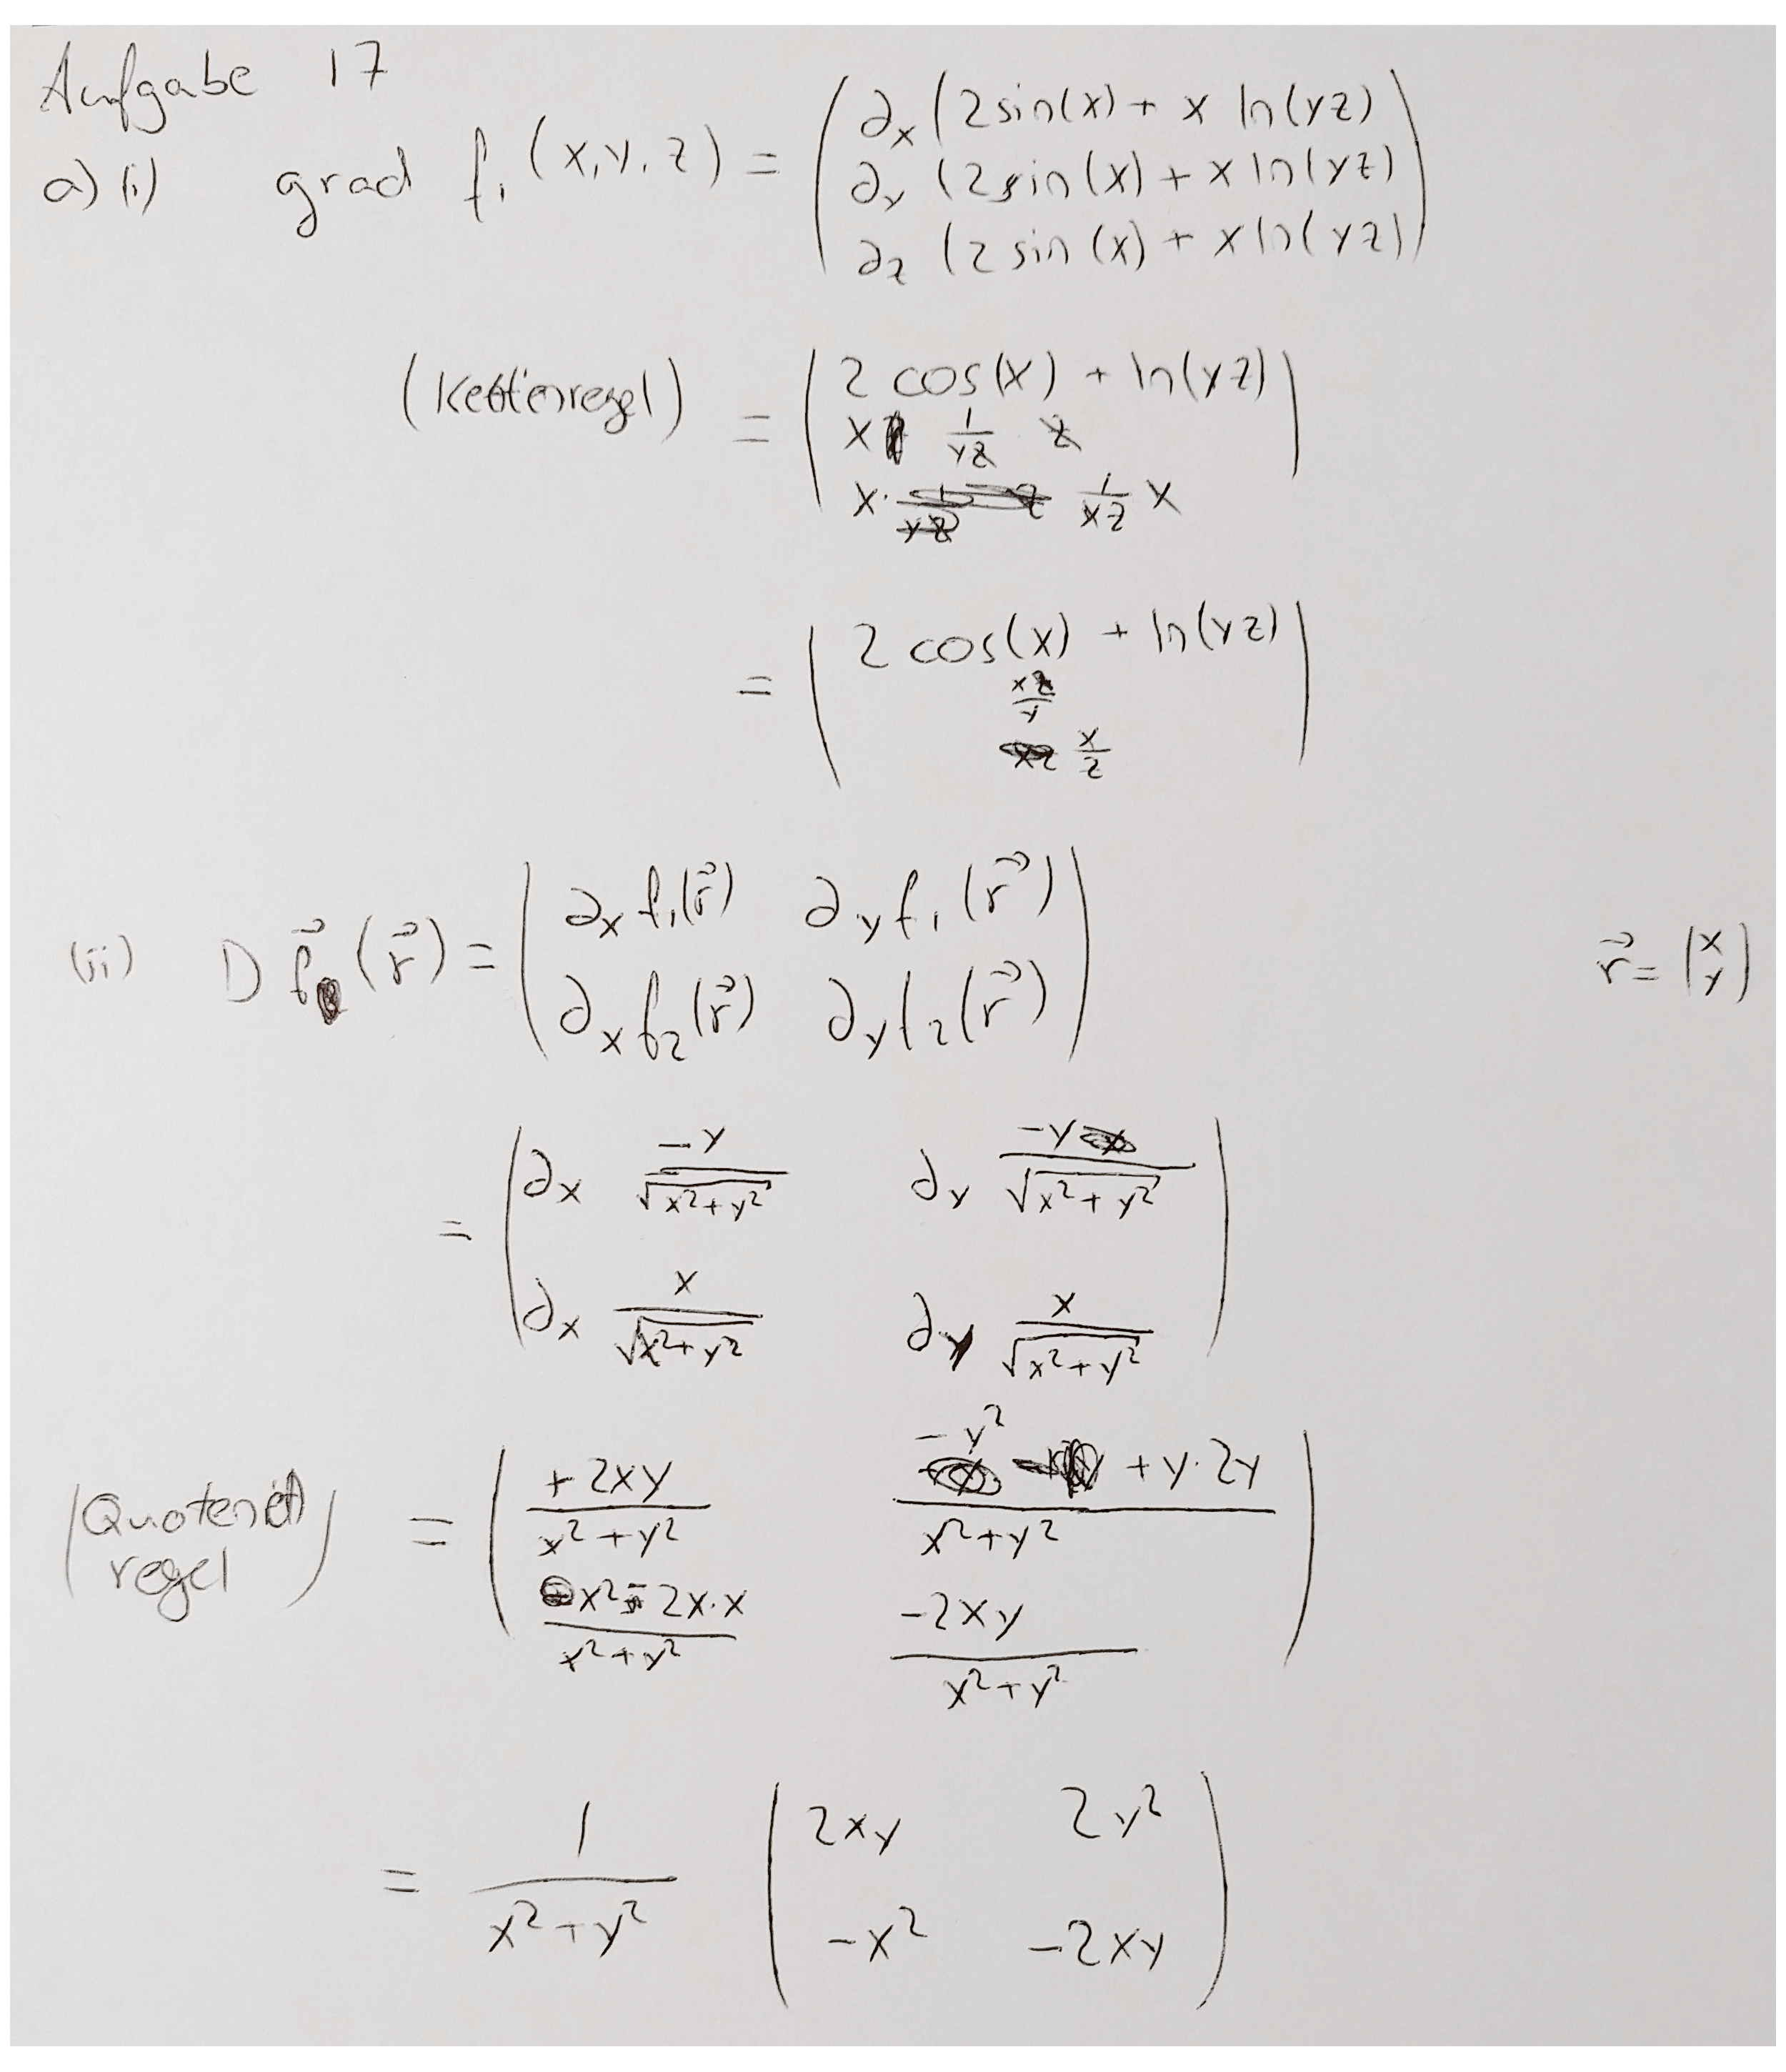
\includegraphics[width=15cm]{17a.png}
\end{figure}

\newpage
\setlength{\headheight}{0cm}
\begin{figure}[H]
	\centering
	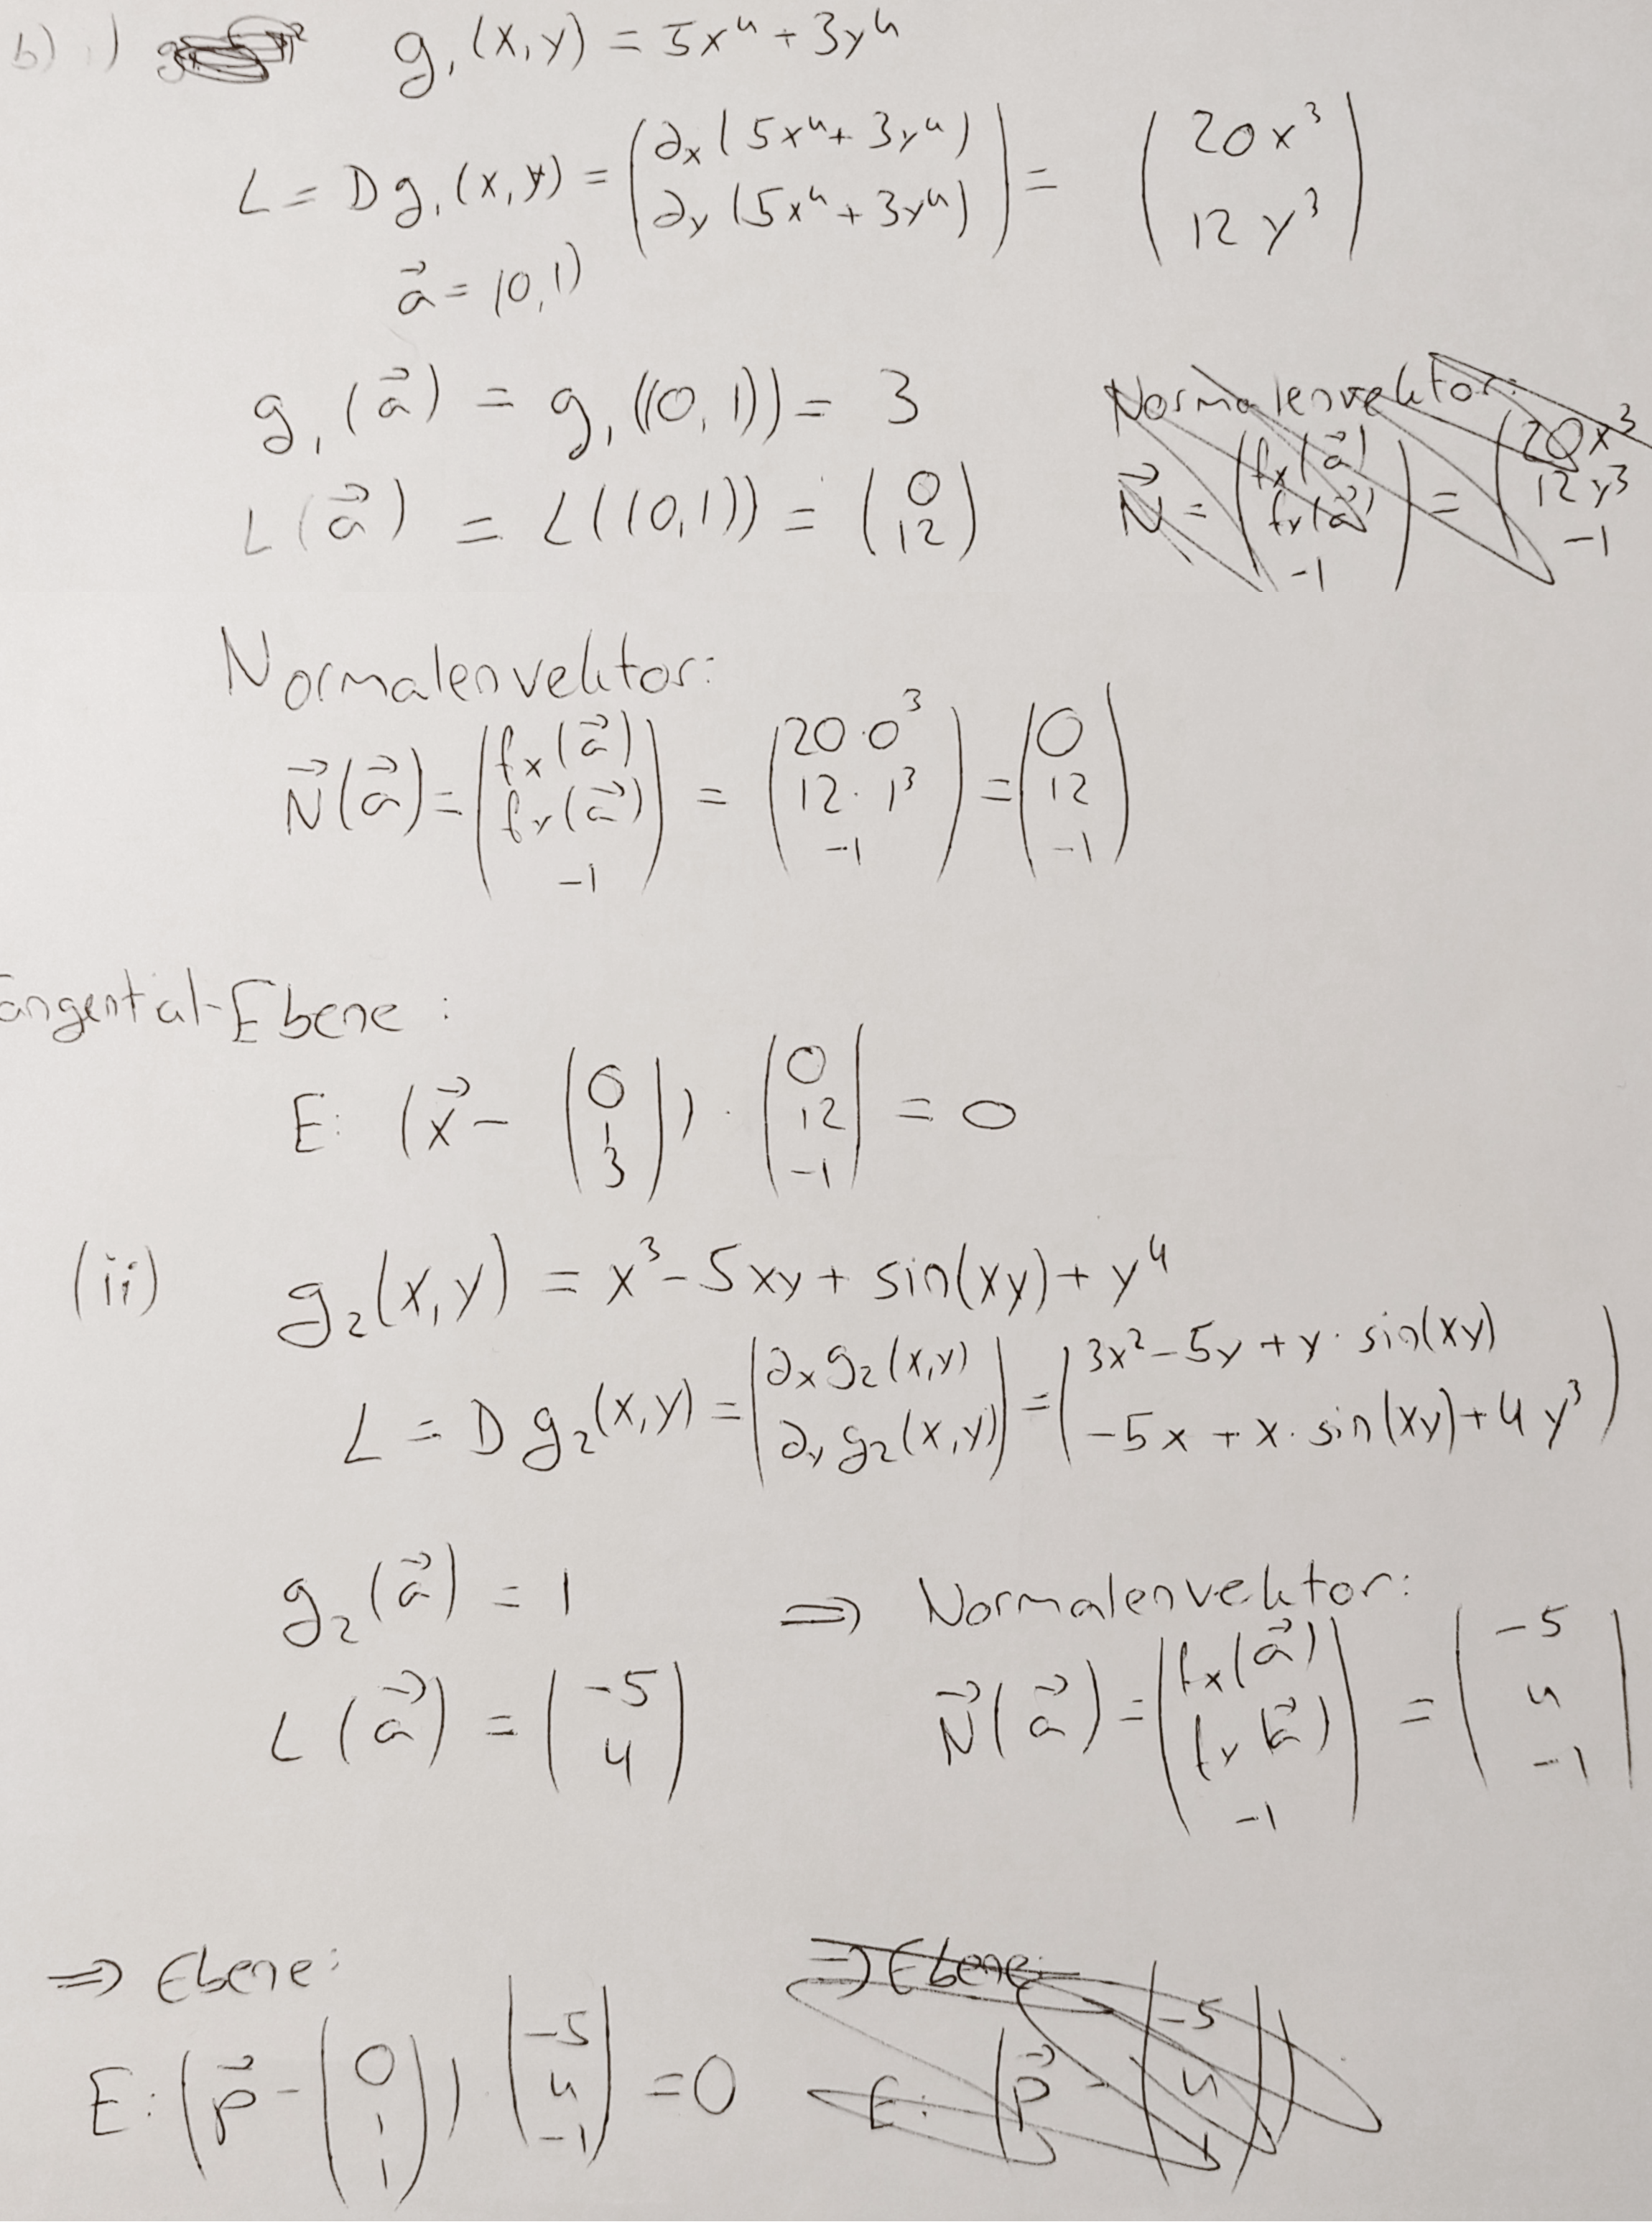
\includegraphics[width=15cm]{17b.png}
\end{figure}

\newpage
\section*{Aufgabe 18}
a) 
\begin{align*}
	D \left(f \vec g\right) (\vec a)
	&= \sum_{i j} \partial_{x_j} \left(f \vec g\right)_i (\vec a) \\
	% produktregel
	^\text{Produkt-}_\text{Regel} \Rightarrow
	&= \sum_{i j} \underbrace{g_i (\vec a)}_{\vec g(\vec a)} 
	\cdot \underbrace{\partial_{x_j} f(\vec a)}_{\nabla f(\vec a)}
	+ f(\vec a) 
	\cdot \underbrace{\partial_{x_j} g_i(\vec a)}_{D\vec g(\vec a)}
	\\
	% zurueck zu normaler notation
	&= \vec g(\vec a) \vec\nabla f(\vec a) + f(\vec a) D\vec g(\vec a)
\end{align*}

b)
\begin{figure}[H]
	\centering
	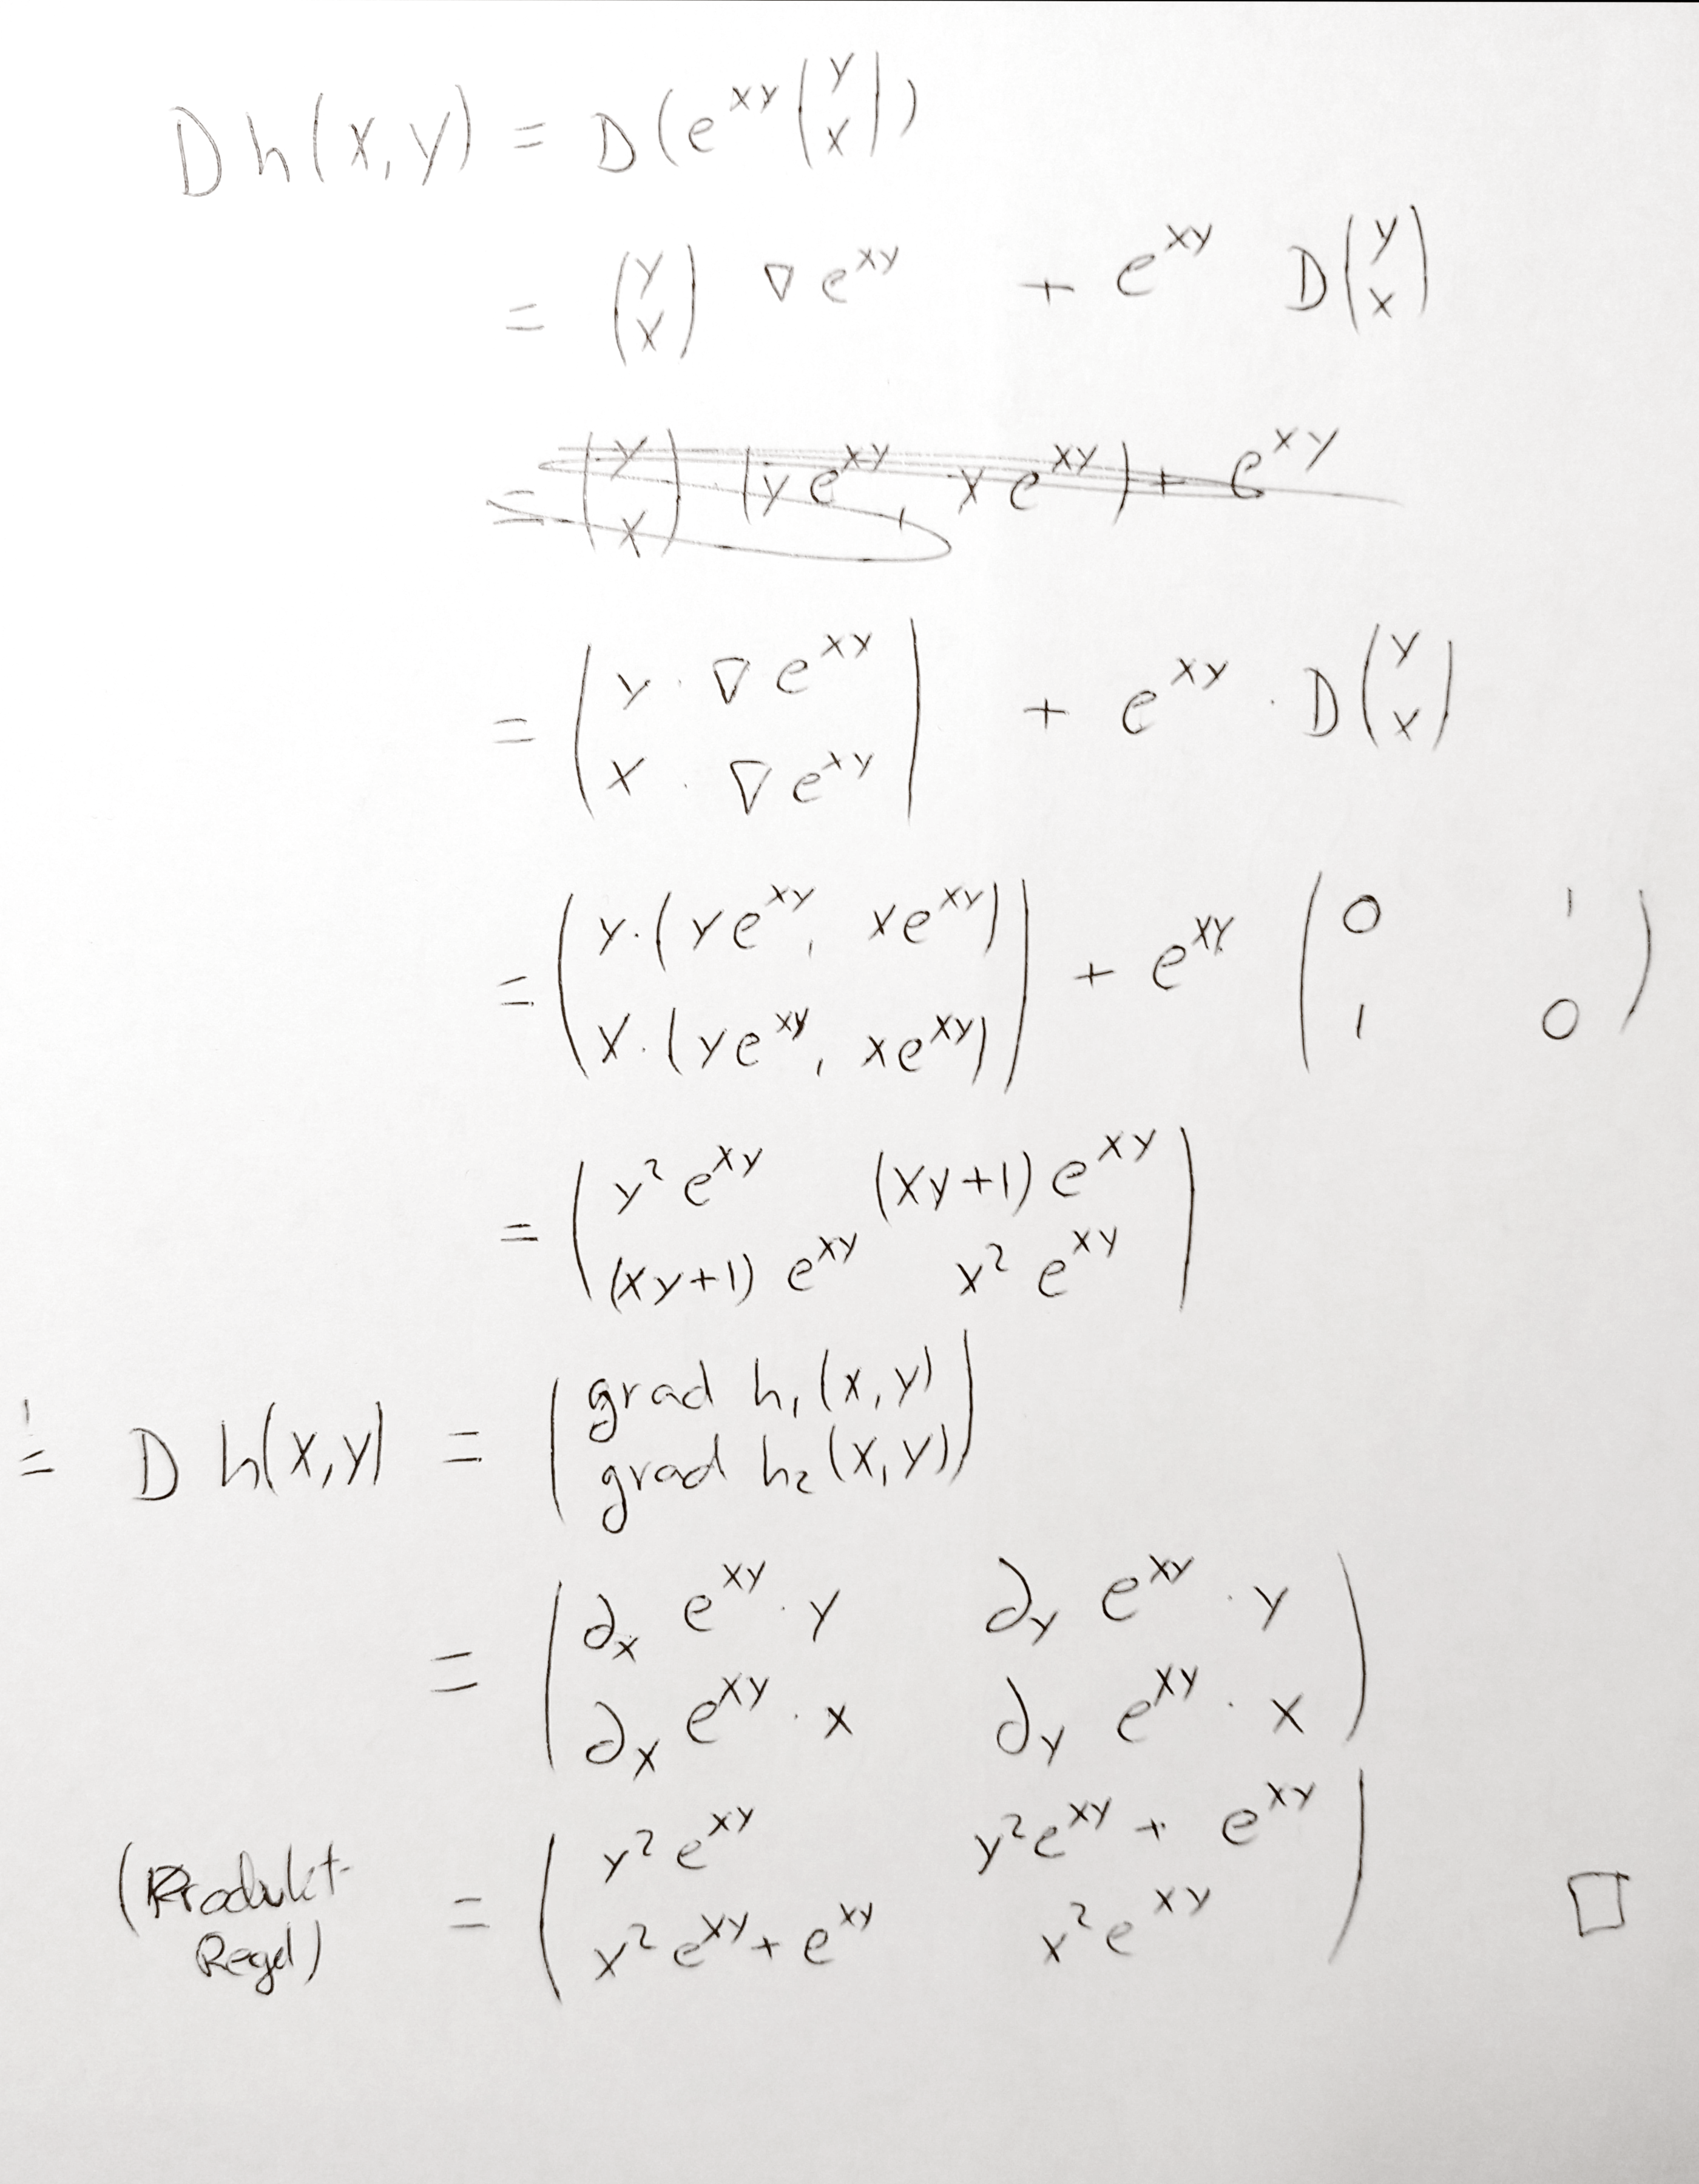
\includegraphics[width=13cm]{18b.png}
\end{figure}

\end{document}
